\apendice{Plan de Proyecto Software}\label{anex:A}

\section{Introducción}
%Ref david goo bees https://github.com/davidmigloz/go-bees puede ayudar con la memoria
Una de las actividades de un proyecto software es la fase de planificación. En esta fase se estima el esfuerzo, el tiempo y el dinero que se espera invertir en el proyecto. El objetivo principal de la fase de planificación es estimar si se puede realizar el proyecto con éxito y, en ese caso, tener una guía de referencia para el proceso de desarrollo. Este anexo recoge los documentos generados en este proceso y se divide en dos partes:
\begin{description}
	\tightlist
	\item Planificación temporal. En esta parte se estima el tiempo y el esfuerzo que se requieren para la realización del proyecto.
	\item Estudio de la viabilidad. Esta parte se estima si el proyecto es viable tanto económica como legalmente, por tanto se dividirá en dos secciones:
	\begin{description}
		\tightlist
		\item[Viabilidad económica]: Análisis del coste y del beneficio que supondría la realización del proyecto.
		\item[Viabilidad legal]: Análisis de las leyes que se aplicarían desde el comienzo del proyecto. En un proyecto software tienen especial importancia las licencias y la Ley de Protección de Datos.
	\end{description}
\end{description}

\section{Planificación temporal}
No se ha realizado una planificación temporal del proyecto. Se han seguido los 12 principios del manifiesto ágil y el modelo SCRUM \cite{noauthor_scrum_2019}:
\begin{itemize}
	\tightlist
	\item Se ha aplicado un desarrollo incremental y evolutivo.
	\item Se han realizado iteraciones (\textit{sprints}) de dos semanas. Al finalizar un sprint se realizaba una reunión entre el tutor y el alumno que daba comienzo al siguiente sprint y que consta de dos partes:
	\begin{itemize}
		\item Una parte de revisión del sprint en la que se exponía una parte operativa del producto realizada durante el sprint.
		\item Otra de planificación del siguiente sprint en la que se determinaba el trabajo y los objetivos a alcanzar durante el siguiente sprint. Esto quedaba reflejado como una pila de tareas que se debían completar durante el sprint y que han sido registradas en el sistema de gestión de incidencias de GitLab.
	\end{itemize}
\end{itemize}
\subsection{Sprints}
A continuación se definen los sprints y sus respectivas pilas de tareas que se llevaron a cabo durante la realización del proyecto. 

Los dos primeros sprints estuvieron dedicados a la investigación y configuración del entorno de desarrollo, se puede observar en la Fig. \ref{fig:M5_Sprints_1_EstudioYConfig}. Por cada sprint se observa su descripción, la fecha de apertura y cierre, y el número de issues asociadas. Y en la Fig. \ref{fig:M5_PrimerasIssues} se muestran las descripciones de las primeras tareas que se definieron, la mayoría etiquetadas como `\textit{Research}' (Estudio o investigación) y `\textit{Project Configuration}' (Configuración del proyecto).

\begin{figure}[!h]
	\centering
	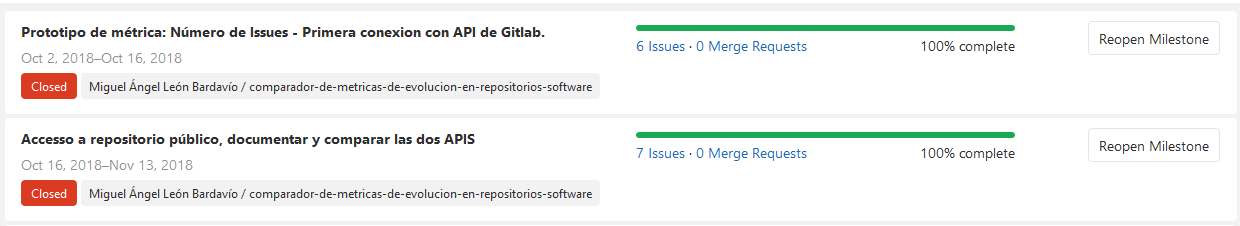
\includegraphics[scale=0.40]{M5_Sprints_1_EstudioYConfig}
	\caption{Milestone iniciales del proyecto en GitLab.}
	\label{fig:M5_Sprints_1_EstudioYConfig}
\end{figure}

\begin{figure}[!h]
	\centering
	\includegraphics[scale=0.40]{M5_PrimerasIssues}
	\caption{Primeras issues del proyecto, la mayoría etiquetadas como `Research' o `Project Configuration'}
	\label{fig:M5_PrimerasIssues}
\end{figure}

Esta etapa de investigación y configuración duró un mes (dos sprints) y sus decisiones afectaron a todo el proyecto. Se recopiló información sobre trabajos relacionados como \textit{Activiti-Api} \cite{rlp0019_software_2019}, \textit{Soporte de Métricas con Independencia del Lenguaje para la Inferencia de Refactorizaciones}  \cite{marticorena_soporte_2005} y \textit{sPACE: Software Project Assessment in the Course of Evolution} \cite{ratzinger_space:_2007} y se estudió los entornos y herramientas que se utilizarían para el desarrollo del proyecto.

Después de esta etapa de investigación, comenzó una etapa de diseño. En esta etapa, las tareas que se definen se relacionan con el diseño de la parte lógica del sistema software a construir, se comienza con la implementación y se empiezan a utilizar las herramientas investigadas anteriormente para construir el sistema. 

Dentro de la fase de diseño se decidió dedicar un tiempo a un tipo de configuración del proyecto que facilitaría el flujo de trabajo y las reuniones de revisión/planificación del sprint. Las principales para mejorar el flujo de trabajo fueron:
\begin{itemize}
	\item Configurar la gestión del proyecto con Maven
	\item Configurar los procesos de integración y despliegue continuo con GitLab (CI/CD)
	\item Realizar pruebas unitarias con JUnit y se automatiza su ejecución gracias a Maven y los \textit{pipelines} de GitLab (CI/CD).
	\item Configurar revisiones automáticas de calidad y de cobertura de las pruebas gracias a Codacy, Jacoco y GitLab.
	\item Configurar un entorno en Heroku donde poder desplegar la aplicación y así poder ser revisada por el tutor fácilmente.
	\item Configurar badges\footnote{} para representar los logros en calidad de código, cobertura, despliegue y los trabajos de CI/CD.
\end{itemize}

Esta etapa de diseño tuvo duración de 3 sprints y uno extra para la configuración del flujo de trabajo, como se puede apreciar en la Fig. \ref{} que muestra los sprints relacionados a esta etapa y en las Figa. \ref{} y \ref{} que muestran las issues relacionadas con la etapa de diseño y la de mejora del flujo de trabajo, respectivamente. Esto se aprecia a que las issues cuentan, en su mayoría con etiquetas `\textit{Design}', excepto las que se refieren al flujo de trabajo que tienen etiquetas como `\textit{Test}', `\textit{Project Configuration}' o `\textit{Question}'.

\begin{figure}[!h]
	\centering
	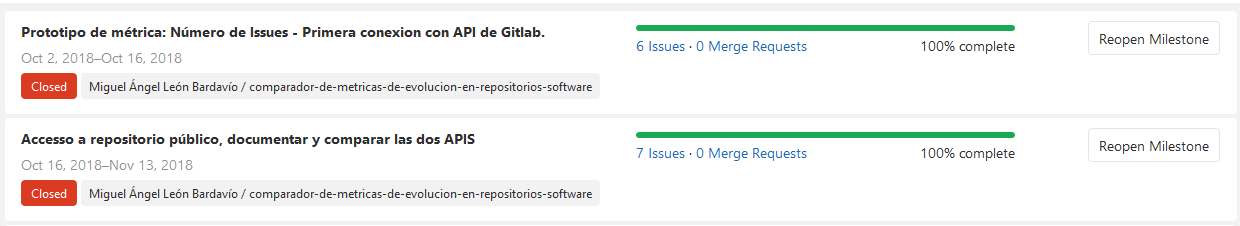
\includegraphics[scale=0.40]{M5_Sprints_1_EstudioYConfig}
	\caption{Milestone iniciales del proyecto en GitLab.}
	\label{fig:M5_Sprints_1_EstudioYConfig}
\end{figure}

\begin{figure}[!h]
	\centering
	\includegraphics[scale=0.40]{M5_PrimerasIssues}
	\caption{Primeras issues del proyecto, la mayoría etiquetadas como `Research' o `Project Configuration'}
	\label{fig:M5_PrimerasIssues}
\end{figure}

\begin{figure}[!h]
	\centering
	\includegraphics[scale=0.40]{M5_PrimerasIssues}
	\caption{Primeras issues del proyecto, la mayoría etiquetadas como `Research' o `Project Configuration'}
	\label{fig:M5_PrimerasIssues}
\end{figure}

\section{Estudio de viabilidad}
\subsection{Viabilidad económica}
En esta sección se realiza un análisis coste-beneficio del proyecto.
\subsection{Viabilidad legal}
En esta sección se realiza un estudio de las leyes que se aplican a este proyecto para asegurar que la realización del proyecto no supondrá ninguna violación de estas leyes. 


